\documentclass{acm_proc_article-sp}
\setlength{\paperheight}{297mm}
\setlength{\paperwidth}{210mm}

\usepackage{txfonts}
\usepackage{cite}
\usepackage{graphicx}
\usepackage{url}
\usepackage{array}
\usepackage{multirow}
\usepackage{color}
\usepackage{booktabs}
\usepackage{float}
\usepackage{lipsum}

\setkeys{Gin}{width=0.98\linewidth}
\graphicspath{{./figures/}}

\IfFileExists{zi4.sty}{\usepackage{zi4}}{\usepackage{inconsolata}}
\usepackage{listings}
\definecolor{bluekeywords}{rgb}{0.13,0.13,1}
\definecolor{greencomments}{rgb}{0,0.5,0}
\definecolor{redstrings}{rgb}{0.9,0,0}
\lstset{language=Java,
	xleftmargin=7mm,
	xrightmargin=2mm,
	frame=single,
	framesep=3pt,
	aboveskip=2em,
	belowskip=1em,
	numbers=left,
	numbersep=9pt,
	captionpos=b,
	tabsize=2,
	keepspaces=true,
	showspaces=false,
	showtabs=false,
	breaklines=true,
	showstringspaces=false,
	breakatwhitespace=true,
	commentstyle=\color{greencomments},
	keywordstyle=\color{bluekeywords},
	stringstyle=\color{redstrings},
	basicstyle=\ttfamily\scriptsize,
	otherkeywords={
		rep,norep,owner,world,any,peer,
		where,reads,writes,pure,impure,
		intersects,disjoint,unique},
	escapeinside={/*@}{@*/}
}

\usepackage{varioref}
\PassOptionsToPackage{pdfpagelabels=false}{hyperref}
\usepackage{hyperref}
\usepackage{cleveref}

\begin{document}

\title{Ownership Types for Local Reasoning}
\subtitle{CS5218: AY2014/2015 Semester 2, Final Project}

\numberofauthors{3} 

\author{
\alignauthor
Darius Foo\\
		\affaddr{A0097282@u.nus.edu}
\alignauthor
Daryl Seah\\
		\affaddr{A0026468@u.nus.edu}
\alignauthor
Joel Low\\
		\affaddr{A0097630@u.nus.edu}
}



\maketitle
\begin{abstract}
The use of ownership types improves local reasoning, allowing both programmers 
and program analysis tools to reason about the correctness and behaviour of 
programs. This would improve the scalability of program analysis tools. This 
paper examines five variations of ownership types, and compares their 
expressiveness as well as their ability to ach\-ieve the goal of improving 
local reasoning. However, owing to the difficulty of annotating programs, it is 
likely that ownership types will only be used for safety-critical programs.
\end{abstract}

\section{Introduction}
\label{sec:introduction}

% Problem, motivation, and Breadth goes here
The advent of Object-Oriented Programming has allowed programmers to write and 
maintain larger components and programs, owing to the modularisation brought 
about by encapsulation. This increased modularisation of programs ought to 
result in a corresponding ease of comprehension for programmers, since 
programmers are now able to reason about programs at a modular level. 
Likewise, it should follow that static program analysis tools be able to 
improve the speed at which analyses can be completed, especially when analysing 
a large program.

\subsection{Limits of Traditional Mechanisms}
label{subsec:traditional\_mechanism\_limits}
In practice, many escape mechanisms which break the encapsulation of an object 
are used. These mechanisms, while allowing expressiveness in programs, prevent 
the programmer from reaping the benefits of being able to isolate a module and 
reason about its behaviour and effects. We present an example in 
\cref{code:modular_reasoning_car_engine_1}, originally 
described in \cite{clarke98ownership}.

\begin{lstlisting}[
	float, floatplacement=t,
	caption={Car},
	label=code:modular_reasoning_car_engine_1
]
class Person {}

class Engine {
	void start() { /* ... */}
}

class Car {
	Engine engine; Person driver;

	void start() {
		if (driver != null) {
			engine.start();
		}
	}
}

class Main {
	static void main() {
		Car car = new Car();
		car.start();
		car.engine.start();/*@\label{code:modular_reasoning_car_engine_1_engine_start}@*/
	}
}
\end{lstlisting}

Here, we present a car, with a driver and an engine. The car defines a 
\lstinline|start| method, which will start the engine; the engine can 
only be started if a driver is present. However, on 
\cref{code:modular_reasoning_car_engine_1_engine_start} the car's engine 
was started, bypassing that check. This should not have been allowed because it 
has broken the encapsulation discipline.

The traditional approach to preventing this is to utilise access specifiers; 
using Java's syntax, there would be four levels of access: \lstinline|public|, 
\lstinline|protected|, \lstinline|private|, and default (package-level) access. 
These access specifiers are annotations on types and variables, limiting 
\emph{visibility} of the identifiers of said types and variables to the 
appropriate scope. \Cref{code:modular_reasoning_car_engine_2}, modified from 
\cref{code:modular_reasoning_car_engine_1}, demonstrates that enforcing 
encapsulation using access specifiers alone are insufficient.

\begin{lstlisting}[
	float, floatplacement=t,
	caption={Car with Access Specifiers},
	label=code:modular_reasoning_car_engine_2
]
class Person {}

class Engine {
	public void start() { /* ... */ }
}

class Car {
	private Engine engine; private Person driver;
	
	public void start() {
		if (driver != null) {
			engine.start();
		}
	}

	public Engine getEngine() { return engine; }
}

class Main {
	public static void main() {
		Car car = new Car();
		car.start();
		car.getEngine().start();/*@\label{code:modular_reasoning_car_engine_2_engine_start}@*/
	}
}

\end{lstlisting}

In Listing~\ref{code:modular_reasoning_car_engine_2} we annotate each method 
and member variable with an appropriate access specifier. We also define an 
additional \emph{accessor} method, for the situation where a property of the 
car's engine must be accessed outside of the car (an instrument attached to the 
car's electronics to measure performance, for example). However, as seen on 
line~\ref{code:modular_reasoning_car_engine_2_engine_start} the original 
problem has not been resolved: the engine can still be started externally. 
There is no way to reconcile access to parts of an object based on who `owns' 
the object, and who is accessing the object. Thus, access specifiers alone are 
not expressive enough.

While access specifiers can be modified to support such a 
scenario\footnote{Read-only and mutable interfaces can be extracted from the 
class, and the appropriate interface returned from methods. This is not common 
practice; however, the Cocoa runtime for Objective-C is notable for doing 
this.}, the resulting API is clumsy because every time a type is defined, 
programmers must manually define the behaviours allowed by mutable and 
immutable references to the object. There would consequently be an explosion of 
types, making reasoning about the program more difficult.

\section{Ownership Types}
\label{sec:ownership}

% terminology and the basics
Ownership Types is an addition to the type system to encode ownership 
information. This directly overcomes the limitations of only using access 
specifiers. Using SafeJava's\cite{boyapati04safejava} syntax, the Car example 
can be expressed as per \cref{code:ownership_types_car_engine_1} 
\vpageref[above]{code:ownership_types_car_engine_1}.

\Cref{code:ownership_types_car_engine_1} introduces the notion of an ownership 
\emph{type}. Just like generics, this is information which is created and 
enforced statically. All types are now parameterised by an ownership type, 
preventing objects with different owners from being assigned (and indeed, 
referenced). Furthermore, it is not possible to express the ownership type of 
an object belonging to another object, preventing the encapsulation violation 
on \cref{code:ownership_types_car_engine_1_engine_start}.

\begin{lstlisting}[
	float, floatplacement=t,
	caption={Car with Ownership Types},
	label=code:ownership_types_car_engine_1
]
class Person {}

class Engine<EngineOwner> {
	void start() { /* ... */ }
}

class Car<CarOwner, DriverOwner> {
	Engine<this> engine; Person<DriverOwner> driver; /*@
		\label{code:ownership_types_car_engine_1_parametric_owner} @*/
	
	void start() {
		if (driver != null) {
			getEngine().start();
		}
	}

	Engine<this> getEngine() { return engine; }
}

class Main {
	static void main() {
		Car<this, world> car = new Car<this, world>();
		car.start();
		car.getEngine().start();/*@\label{code:ownership_types_car_engine_1_engine_start}@*/
	}
}
\end{lstlisting}

Ownership parameters can also be used within the class declaration, as shown on 
\cref{code:ownership_types_car_engine_1_parametric_owner}. Special keywords 
have been introduced: \lstinline|world| indicating that the value is not owned 
by any object (i.e. it is owned by the system), and \lstinline|this| has been 
overloaded to mean the current object's ownership context.

Type-checking this program results in a type-check failure because it is not 
possible to express the ownership context of the car outside of the class. 
However, it is possible to express the car's ownership to objects used by it, 
through the ownership parameter mechanism.

This is one of the few approaches that we have examined. The other approaches 
are conceptually similar; the difference among them lies mainly in their 
expressivity.

\subsection{Definitions}
\label{subsec:definitions}

In this paper, we try to make our definitions as generic as possible, allowing 
a consistent set of terms to be used across the different systems proposed.

\begin{description}
	\item[Expressivity] How complex a notion of ownership a system can allow a 
	programmer to express. We have designed various use cases, which encompass 
	a variety of design patterns which can be found in programs used today, and 
	analysed each system for its ability to express such a design pattern. Our 
	use cases can be broadly categorised as such:
	
	\begin{itemize}
		\item \textbf{Abstract Data Types}: We modified a Queue example from 
		\cite{boyapati04safejava}, and added iterators, which can be seen as a 
		view over the data stored in the data type.
		\item \textbf{Inheritance}: A recurring pattern in Object-Oriented 	
		Programming where behaviour is augmented onto existing classes.
		\item \textbf{Generics}: Building upon the ADT use case, Generics 
		allow 	
		programmers to write reusable components.
		\item \textbf{Cardinality of Ownership}: Having multiple owners of an 
		object is useful for writing parallel/distributed algorithms.
		\item \textbf{Ownership Transfer}: Allowing the transfer of ownership 
		from 
		one object to another is useful for producer-consumer pattern.
		
	\end{itemize}
	
	\item[Representation Invariant] A constraint on the state of the object, 
	maintained throughout its lifetime
	\item[Owner] An object or objects responsible for maintaining  the 
	representation invariant of an object.
	\item[Context \emph{a.k.a. Universe, Box}] A nested partition of the object 
	store containing all the objects constituting the representation of 
	a particular object.

\end{description}

\subsection{Ownership Topologies}
\label{subsec:topologies}

An ownership topology is a description of the structure and organisation of the 
object store. In this paper, two topologies are examined:

\begin{description}
	\item[Hierarchical \emph{a.k.a. Tree}] This is a single ownership topology, 
	where every object as one owner.
	\item[Directed Acyclic Graph (DAG)] This is a multiple ownership topology, 
	where an object can have multiple owners. All owners of the object can 
	modify its invariant.
\end{description}

\subsection{Encapsulation Disciplines}
\label{subsec:encapsulation}

Where an ownership topology \emph{describes} the structure of the object store, 
an encapsulation discipline \emph{prescribes} the structure of the object 
store. They can thus be seen as related ideas. In this paper, two main 
encapsulation disciplines are discussed:

\begin{description}
	\item[Owners-as-Dominators] Objects can only be modified by following a 
	reference chain from the root context through the object's owner. Aliasing 
	is restricted, because no aliases to an object B owned by an object A can 
	exist outside of the ownership context of object A.
	\item[Owners-as-Modifiers] Objects can only be modified by following a 
	reference chain from the root context through the object's owner. However, 
	read-only access is granted in all other contexts. Aliasing is \emph{not} 
	restricted.
	
\end{description}

\subsection{Applications}
\label{subsec:apps}

\lipsum[5]




\section{Variants}
\label{sec:variants}

\lipsum[6]

\subsection{Clarke's Ownership Types}
\label{subsec:clarke}

\lipsum[7]

\subsection{Boyapati's SafeJava}
\label{subsec:boyapati}

\lipsum[8]

\subsection{Dietl and M\"{u}ller's Universe Types}
\label{subsec:dietl}

\lipsum[9]

\subsection{Cameron's Multiple Ownership}
\label{subsec:cameron}

\lipsum[10]



\section{Evaluation}
\label{sec:eval}

\lipsum[11]




\section{Conclusion}
\label{sec:conclude}

\lipsum[12]


\newcommand{\col}[1]{ }

\begin{table*}[t]
\caption{Expressivity of Ownership Types.}
\label{tab:expressivity}
\centering
\renewcommand{\arraystretch}{1.3}
\footnotesize
\begin{tabular}{ccccc}
\toprule
& & & ~\textbf{Generic}~ & \\
~\textbf{Original}~ & ~\textbf{SafeJava}~ & 
~\textbf{Universe Types}~ & ~\textbf{Universe Types}~ & ~\textbf{Multiple Ownership}~\\
\midrule
1		& 39		& 3	& 5.65	\\
2		& 47		& 4	& 7.01	\\
3 		& 53		& 3	& 9.71	\\
1 \& 2	& 86		& 4	& 8.13	\\
2 \& 3	& 100	& 4	& 9.48	\\
1, 2 \& 3	& 139	& 5	& 9.35	\\
\bottomrule
\end{tabular}
\end{table*}

% clarke98ownership
% boyapati04safejava
% cunningham08ut
% dietl11gut
% cameron07mojo

$\medbullet$
$\medcirc$
$\otimes$




\section{Testing}
\label{sec:test}

% Code Snippets
\begin{lstlisting}[
	float, floatplacement=t,
	caption={Car Engine Example},
	label=code:car_eng_test
]
class Person {}
class Engine<any engineOwner> {
  void start() { /* ... */ }
}

class Car<carOwner, driverOwner> {
  Engine<this> engine; Person<a & ?> driver;
    
  void start() {
    if (driver != null) getEngine().start();
  }
  Engine<world> getEngine() { return engine; }
}
\end{lstlisting}

% Figures
\begin{figure}[t]
\centering
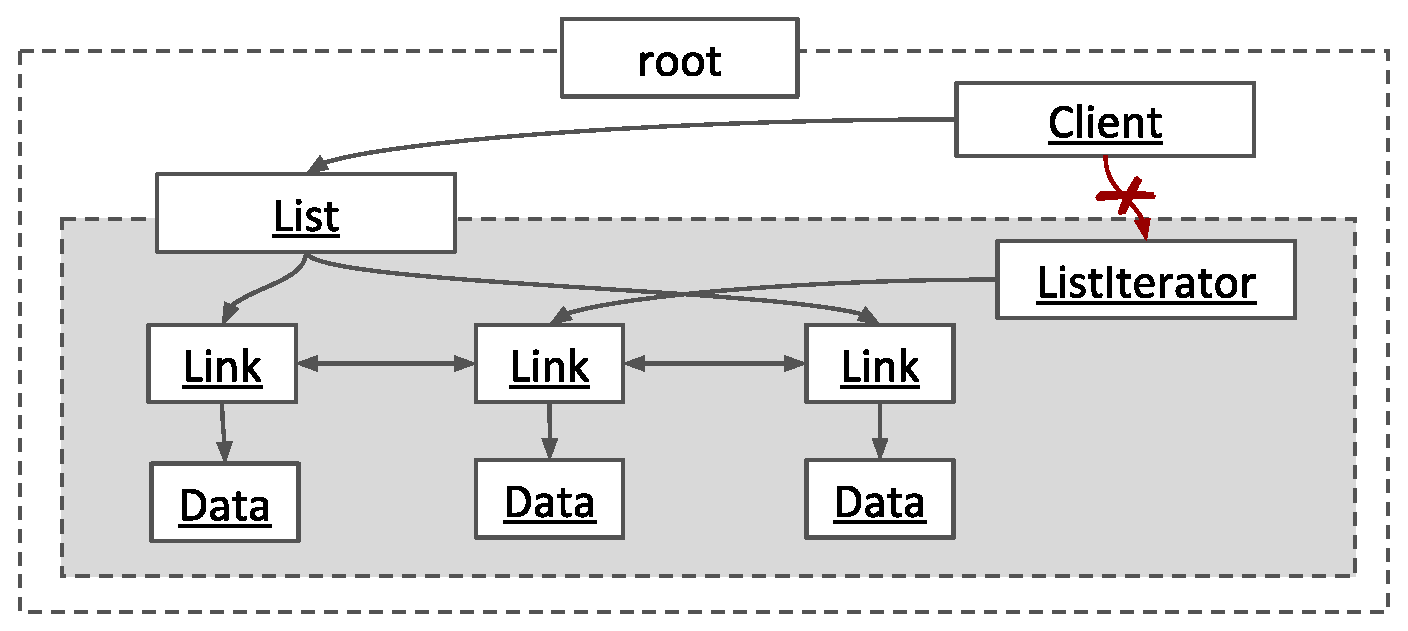
\includegraphics{iterator-fail-inside.eps}
\caption{List Iterator inside representation.}
\label{fig:iterator-inside-test}
\end{figure}

\begin{figure}[t]
\centering
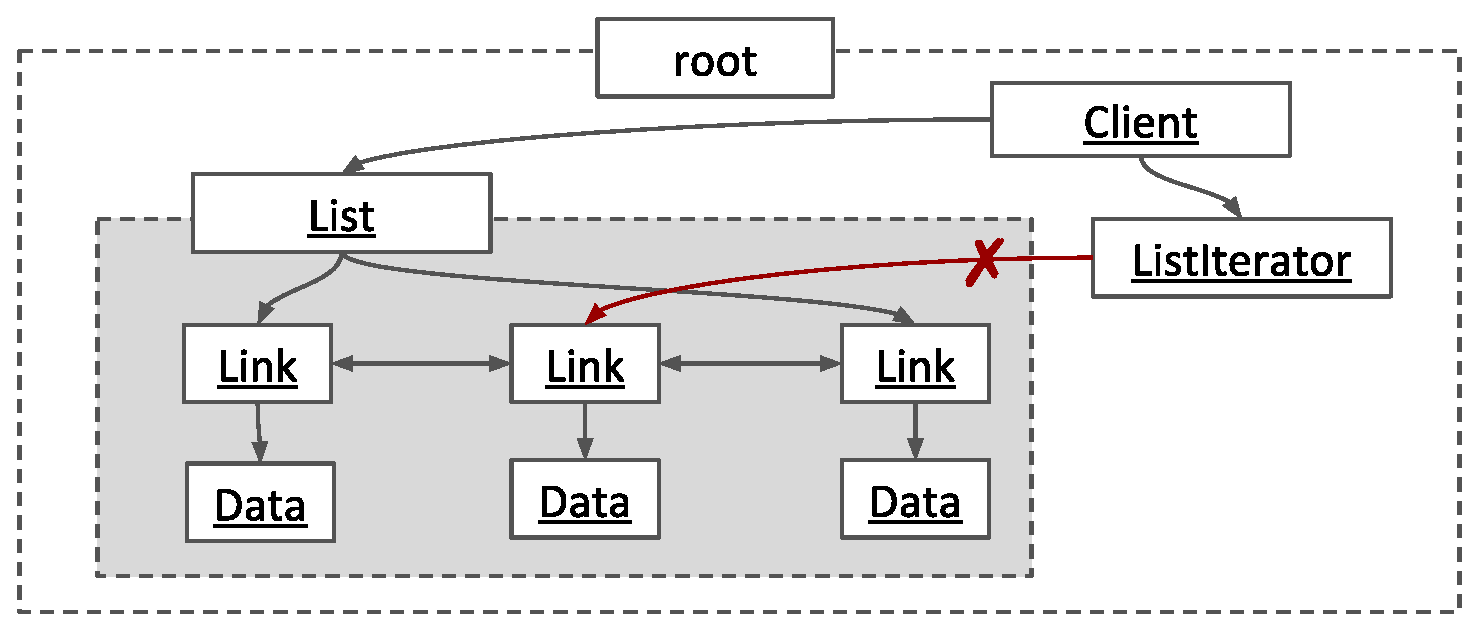
\includegraphics{iterator-fail-outside.eps}
\caption{List Iterator outside representation.}
\label{fig:iterator-outside-test}
\end{figure}

Reference to \cref{code:car_eng_test}, \cref{sec:test} and 
\cref{fig:iterator-inside-test,fig:iterator-outside-test}.

% Citations
aldrich04domains~\cite{aldrich04domains},\newline
aldrich02aliasjava~\cite{aldrich02aliasjava},\newline
almeida97balloons~\cite{almeida97balloons},\newline
boyapati04safejava~\cite{boyapati04safejava},\newline
boyapati02races~\cite{boyapati02races},\newline
boyapati03innerclass~\cite{boyapati03innerclass},\newline
boyapati03rtsj~\cite{boyapati03rtsj},\newline
cameron07mojo~\cite{cameron07mojo},\newline
cameron10encoding~\cite{cameron10encoding},\newline
clarke03ownership~\cite{clarke03ownership},\newline
clarke02ownership~\cite{clarke02ownership},\newline
clarke13aliasing~\cite{clarke13aliasing},\newline
clarke98ownership~\cite{clarke98ownership},\newline
cunningham08ut~\cite{cunningham08ut},\newline
dietl09gut~\cite{dietl09gut},\newline
dietl11gut~\cite{dietl11gut},\newline
dietl07gut~\cite{dietl07gut},\newline
dietl13ownership~\cite{dietl13ownership},\newline
dietl08dependent~\cite{dietl08dependent},\newline
dietl05jml~\cite{dietl05jml},\newline
hogg91islands~\cite{hogg91islands},\newline
muller02modular~\cite{muller02modular},\newline
muller99universes~\cite{muller99universes},\newline
noble98alias~\cite{noble98alias}



\bibliographystyle{abbrv}
\bibliography{report}

\end{document}
